\documentclass[12pt,a4paper,notitlepage]{article}
\usepackage[utf8]{inputenc}
\usepackage[english]{babel}
\usepackage[T1]{fontenc}
\usepackage[backend=biber,
			style=authoryear-comp,
			isbn=false,
			doi=false,
			bibstyle=authoryear,
			natbib,
			]{biblatex}
\usepackage{eurosym}
\usepackage{enumitem}
\usepackage{url}
\usepackage{blindtext}
\usepackage{hyperref}
\usepackage{breakurl}
\usepackage{amsmath}
\usepackage{titling}
\usepackage{amsfonts}
\usepackage{amssymb}
\usepackage{pgfplots}
\usepackage{caption}
\usepackage{subcaption}
\usepackage{graphicx}
\usepackage{dcolumn}
\usepackage{tikz-3dplot}
\usepackage{subcaption}
\usepackage{float}
\usepackage{adjustbox}
\usepackage{multirow,rotating}
\usepackage[autostyle]{csquotes}
\usepackage[toc,page]{appendix}
\usepackage{lscape}
\usepackage{todonotes}
\usepackage{booktabs}
\usepackage{multirow}
\usepackage{bm}
\usepackage{eurosym}

\begin{document}

\section{Introduction}

Social networks such as Facebook are becoming more and more important for online news services: an increasing number of their readers access the news pages via links in the networks. Users of Facebook, for example, can use their profile to share links to external websites - such as news portals - with their online friends. This has led to the development of social media becoming an important generator of traffic for content providers. In Germany, 94\% of online shared news articles in 2015 are distributed via Facebook, followed by Twitter with 3.5\% and Google+ with 2.3\% \citep{schiller_development_2016}. 

The advertising-financed business model of the media houses is based on the premise that users visit their websites in order to achieve high advertising revenues. For this reason, news agencies are particularly interested in finding out which topics are more likely shared on these platforms. \citet{schiller_development_2016} show, that social media users choose a certain site depending on the researched topic. FOCUS Online for example is targeted for articles from politics and business, while sports news is more likely to be shared from Bild.de. 

While these pre-defined resorts give an indication on the content of an article, multiple articles in the same resort probably don't cover the same topics. Especially if the articles originate from different news portals. Furthermore, articles can contain more than one topic. We use a structural topic model to reveal the underlying topics of a collection of articles, and how the articles exhibit them. We then estimate the effect of topic prevalence on the number of Facebook shares. 

Mapping raw text to one or more topics, without having prior knowledge on what those topics are, translates to an unsupervised classification problem on natural language. Topic models generate low-dimensional representations of data and can uncover interesting latent structure in large text datasets. They are popular tools for automatically identifying prominent themes in text. Within topic models the Latent Dirichlet Allocation (LDA) is a widely used technique, where each document (article) is viewed as a mixture of topics (represented by the document-topic distribution) and each topic is a mixture of unique terms, represented by the topic-term distribution \citep{blei_latent_2003}. \citet{roberts_model_2016} extents the base idea of LDA by developing a structural topic model (STM) that allows to incorporate external variables that effect both topical content and topical prevalence. We use this approach to analyze online news about the german federal elections, where we allow prevalence of topics to vary across newswire services. We then estimate the effect of topical prevalence (the posterior document-topic distribution) on the number of Facebook shares.

Figure \ref{fig_research_strat} gives an overview of the applied research strategy. Chapter \ref{ch_model} explains the generative process of the mixed membership model and the results of this process are presented in chapter \ref{ch_results}. Chapter \ref{ch_data} contains a description of the text data and how it was pre-processed in order to use it as input variable.  Chapter \ref{ch_regression} describes how we regress the estimated probabilities of topic prevalence of a document on the times, this document was shared on Facebook.

\begin{figure}[ht]
	\centering
	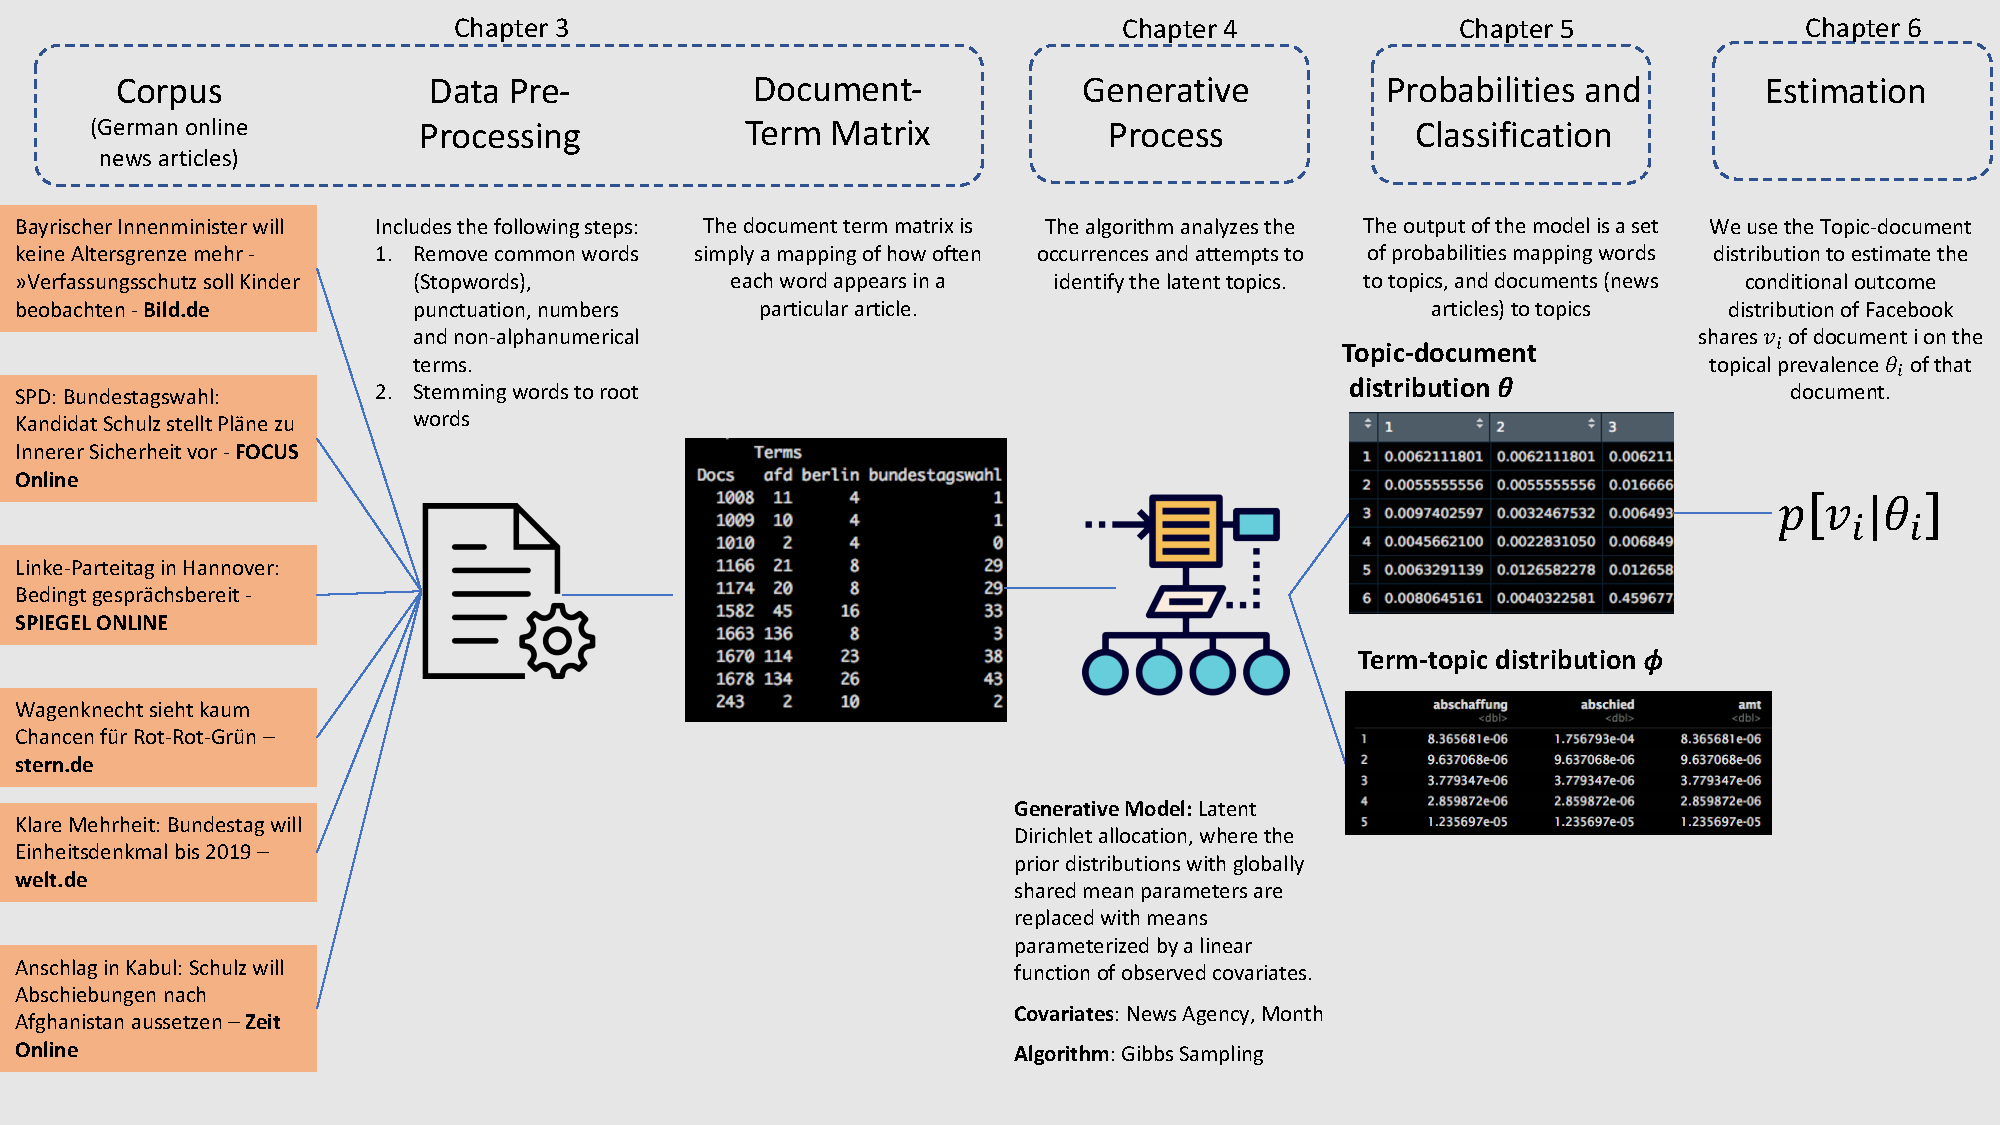
\includegraphics[width=0.95\textwidth]{../figs/research_strategy.pdf} 
	\caption{Research Strategy}
	\label{fig_research_strat}
\end{figure}

% Related Literature
% ------------------

\section{Related Literature}

% Quantitative approaches
% -----------------------


% Topic Modeling / LDA
% ---------------------------

Topic modeling is a statistical and computational technique for discerning information about the contents of a large corpus of documents without reading or annotating the original texts. A topic model uncovers patterns of word co-occurrence across the corpus, yielding a set of word clusters, together with associated probabilities of occurrence, which constitute the topics.

See \citep{taddy_estimation_2012} for a review of topic estimation techniques)

Since its introduction into text analysis, topic modeling has become hugely popular.8 (See \citet{blei_probabilistic_2012} for an overview.) The model has been especially useful in political science (e.g., \citep{grimmer_bayesian_2010}), where researchers have been successful in attaching political issues and beliefs to the estimated latent topics.

Topic modeling is alternatively labeled as “latent Dirichlet allocation,” (LDA) which refers to the Bayesian model in \citet{blei_latent_2003} that treats each $\boldsymbol{v}_i$ and $\boldsymbol{\theta}_l$ as generated from a Dirichlet - distributed prior.
The same model was independently introduced in genetics by \citet{pritchard_inference_2000} for factorizing gene expression as a function of latent populations; it has been similarly successful in that field. 

The basic topic model has been generalized and extended in variety of ways. A prominent example is the dynamic topic model of \citet{blei_dynamic_2006}, which considers documents that are indexed by date (e.g., publication date for academic articles) and allows the topics, say $\boldsymbol{\Theta}_t$, to evolve smoothly in time. 

Applications:


% Structural topic models (STM)
% ----------------------------
A typical application of topic modeling in the social sciences first estimates LDA, then uses estimates of $\theta_d$ as the dependent variable in an regression on covariates to test whether different types of documents have different content. 

This is contradictory because documents are assumed to be generated by a statistical process that we subsequently reject.

The structural topic model (STM) of Roberts et. al. (2016) explicitly introduces covariates into a topic model, and allows one to estimate the impact of document-level covariates on topic content and prevalence as part of the topic model itself.

Applications:
Structural topic modeling is an alternative to LDA that allows researchers to link topics to covariate data and to model changes in topic prevalence over time. STM has recently been applied to scientific texts on climate change, revealing links between corporate funding and the framing of scientific studies \citep{farrell_corporate_2016}. It has also been applied to social media data in a variety of ways. One study shows that “STM can be used to detect significant events such as the downing of Malaysia Air Flight 17” when applied to twitter data \cite{mishler_using_2015}. Another study shows how STM can be used to explore relatively large data sets including course evaluations and discussion forum posts from a Massive Open Online Course \cite{reich_computer-assisted_2014}. 

\cite{roberts_structural_2014} . This article focuses on how the STM is helpful for survey researchers and experimentalists. The STM makes analyzing open-ended responses easier, more revealing, and capable of being used to estimate treatment effects. We illustrate these innovations with analysis of text from surveys and experiments.

\cite{lucas_computer_2015} This article discusses practical issues that arise in the processing, management, translation, and analysis of textual data with a particular focus on how procedures differ across languages. These procedures are combined in two applied examples of automated text analysis using the recently introduced Structural Topic Model. We also show how the model can be used to analyze data that have been translated into a single language via machine translation tools. All the methods we describe here are implemented in open-source software packages available from the authors.

\citet{baturo_what_2017} applies STM to countries’ annual statements in the UN General Debate. This paper identifies the main international development topics that states raise in these speeches between 1970 and 2016, and examine the country-specific drivers of international development rhetoric.

\cite{das_trends_2017} Through the use of a structural topic model, this study introduced distinct topic models on the basis of the relative frequencies of the words used in the abstracts of 15,357 TRB compendium papers. With data from 7 years (2008 through 2014) of TRB annual meeting compendium papers, the 20 most dominant topics emerged from a bag of 4 million words. 

\cite{law_constitutional_2016}  analysis of the world’s constitutional preambles using methods from computational linguistics suggests that they consist of a combination of the three archetypes. Estimation of a structural topic model yields a quantitative measure of the extent to which each preamble draws upon each archetype.

\cite{mueller_reading_2016} This article provides a new methodology to predict armed conflict by using newspaper text. They use the estimated topic shares in linear fixed effects regression to forecast conflict out-of-sample.
 
% -----
% Data
% -----

\section{Dataset}\label{ch_data}

We conduct our estimation on a sample of 10531 news articles containing the term "Bundestagswahl" (Federal Election) dated from 01.06.2017 to 28.10.2017.\footnote{German federal elections took place on 24th of September 2017.} We first extract all online articles of six mainstream german online news portals\footnote{Bild.de, Focus.de, Spiegel.de, Stern.de, Welt.de, Zeit.de} using the the Event Regestry API.\footnote{For more information see http://eventregistry.org/documentation. The scraping code was written in Python and can be made available on request.} We then filter those articles that contain the term "Bundestagswahl" (Federal Election) in their text body. We use the URL of these articles, to check how many times they where shared on Facebook using the \textit{sharedcount} API.\footnote{http://docs.sharedcount.com/}

Figure \ref{fig_distr1} shows the distribution of the number of articles from the respective news sources by date. There is a high peak around the federal elections on September, 24th. Most of the articles are published by welt.de, followed by stern.de (see \ref{fig_distr2}).  

\begin{figure}[H]
	\caption{Article distribution...}
	\begin{center}
		\begin{subfigure}[normla]{0.49\textwidth}
			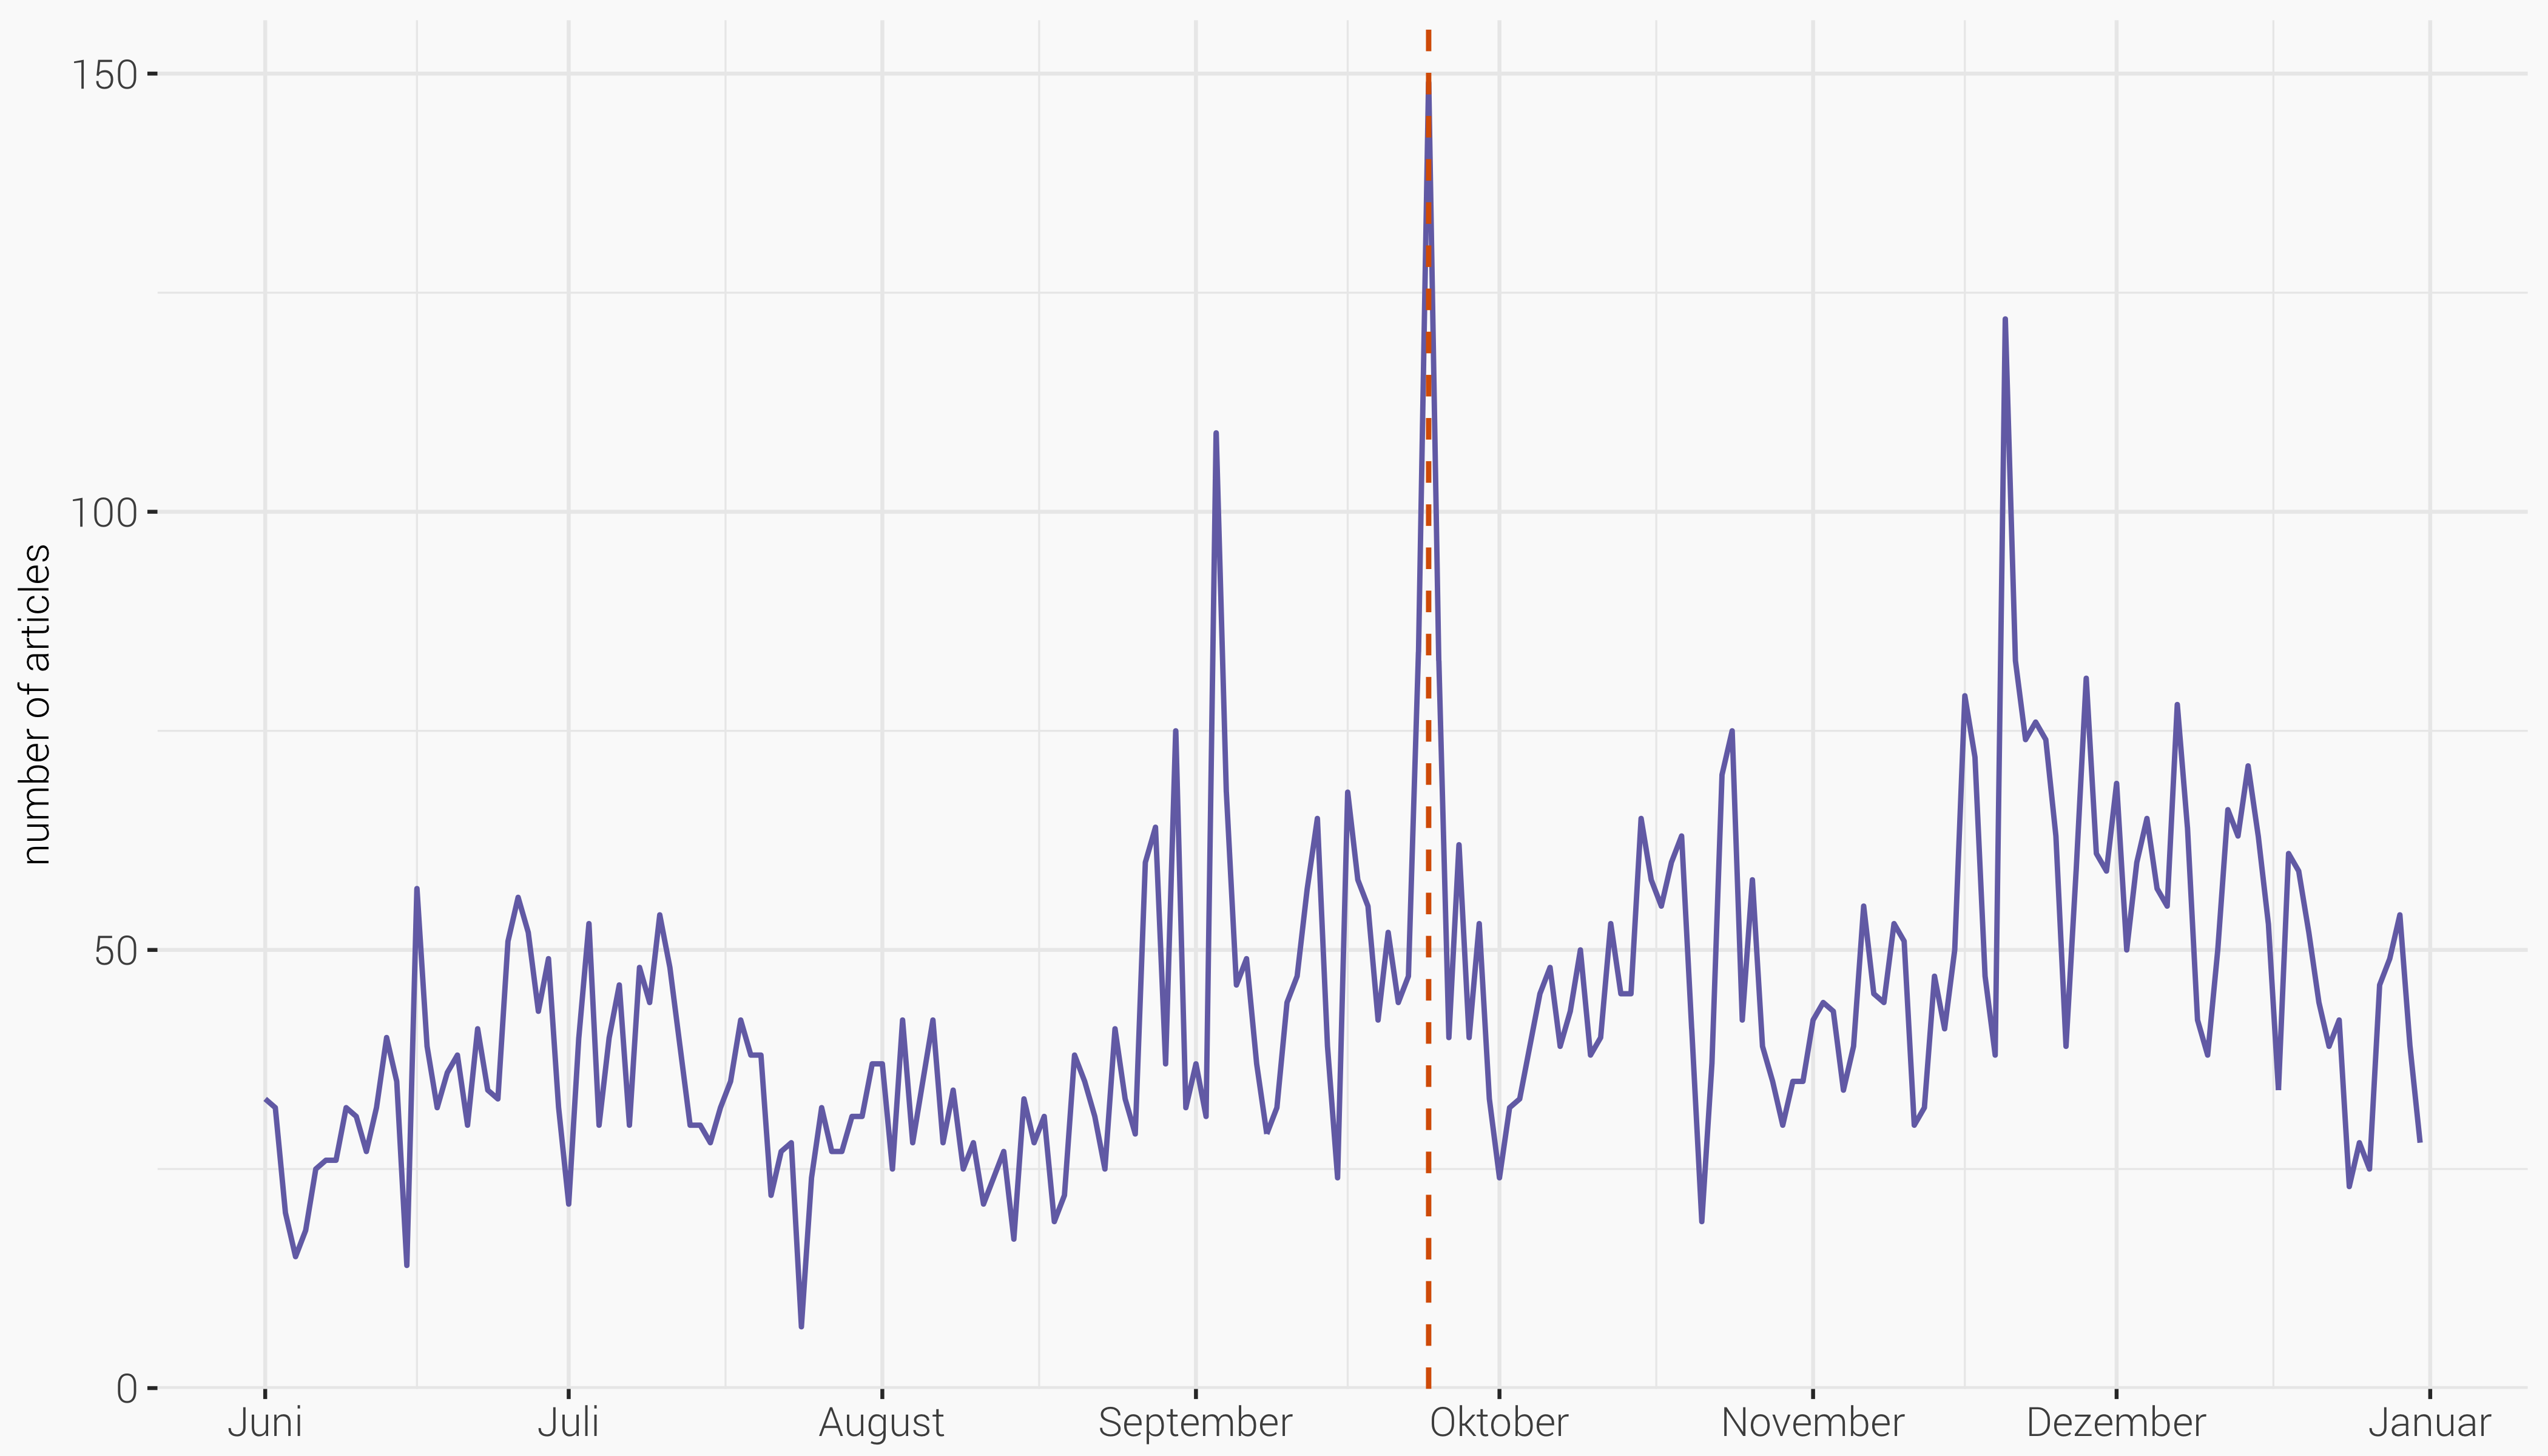
\includegraphics[width=\textwidth]{../figs/timeline.png}
			\caption{...by date \& news source}
			\label{fig_distr1}
		\end{subfigure}
		\begin{subfigure}[normla]{0.49\textwidth}
			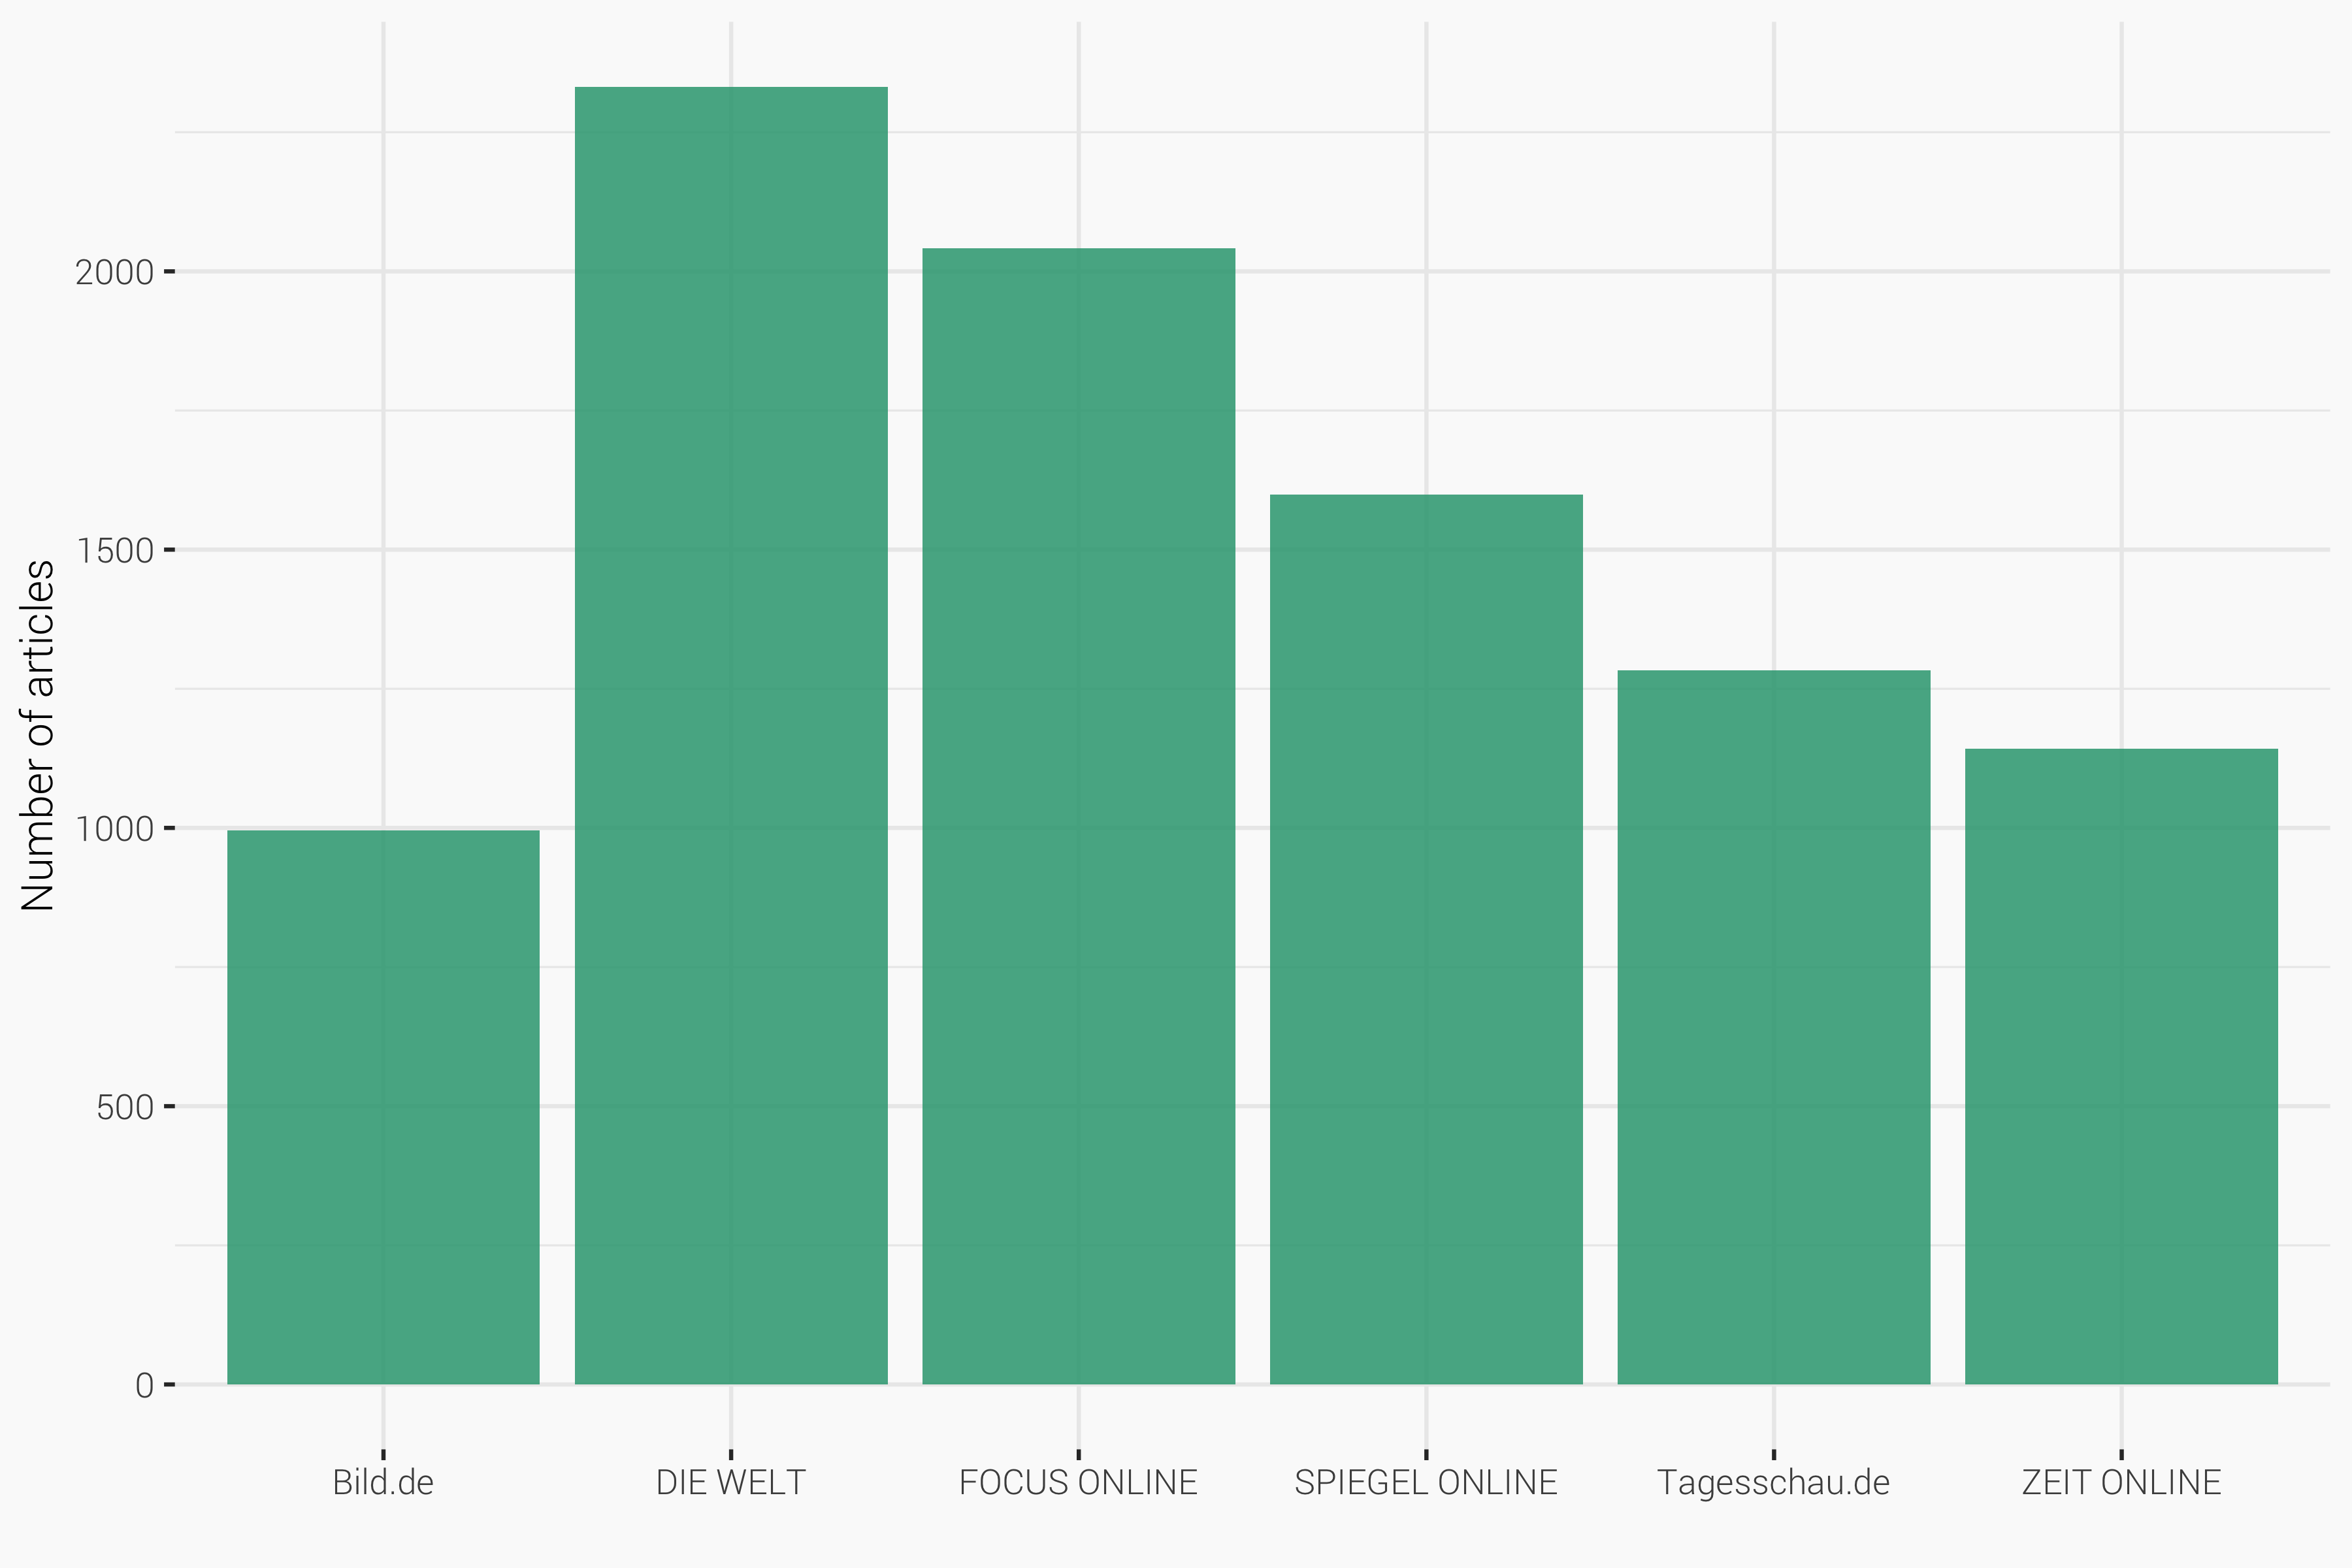
\includegraphics[width=\textwidth]{../figs/bar.png}
			\caption{... by news source}
			\label{fig_distr2}
		\end{subfigure}
	\end{center}
\end{figure}

\begin{figure}[H]
	\caption{Distribution of Facebook shares...}
	\begin{center}
		\begin{subfigure}[normla]{0.49\textwidth}
			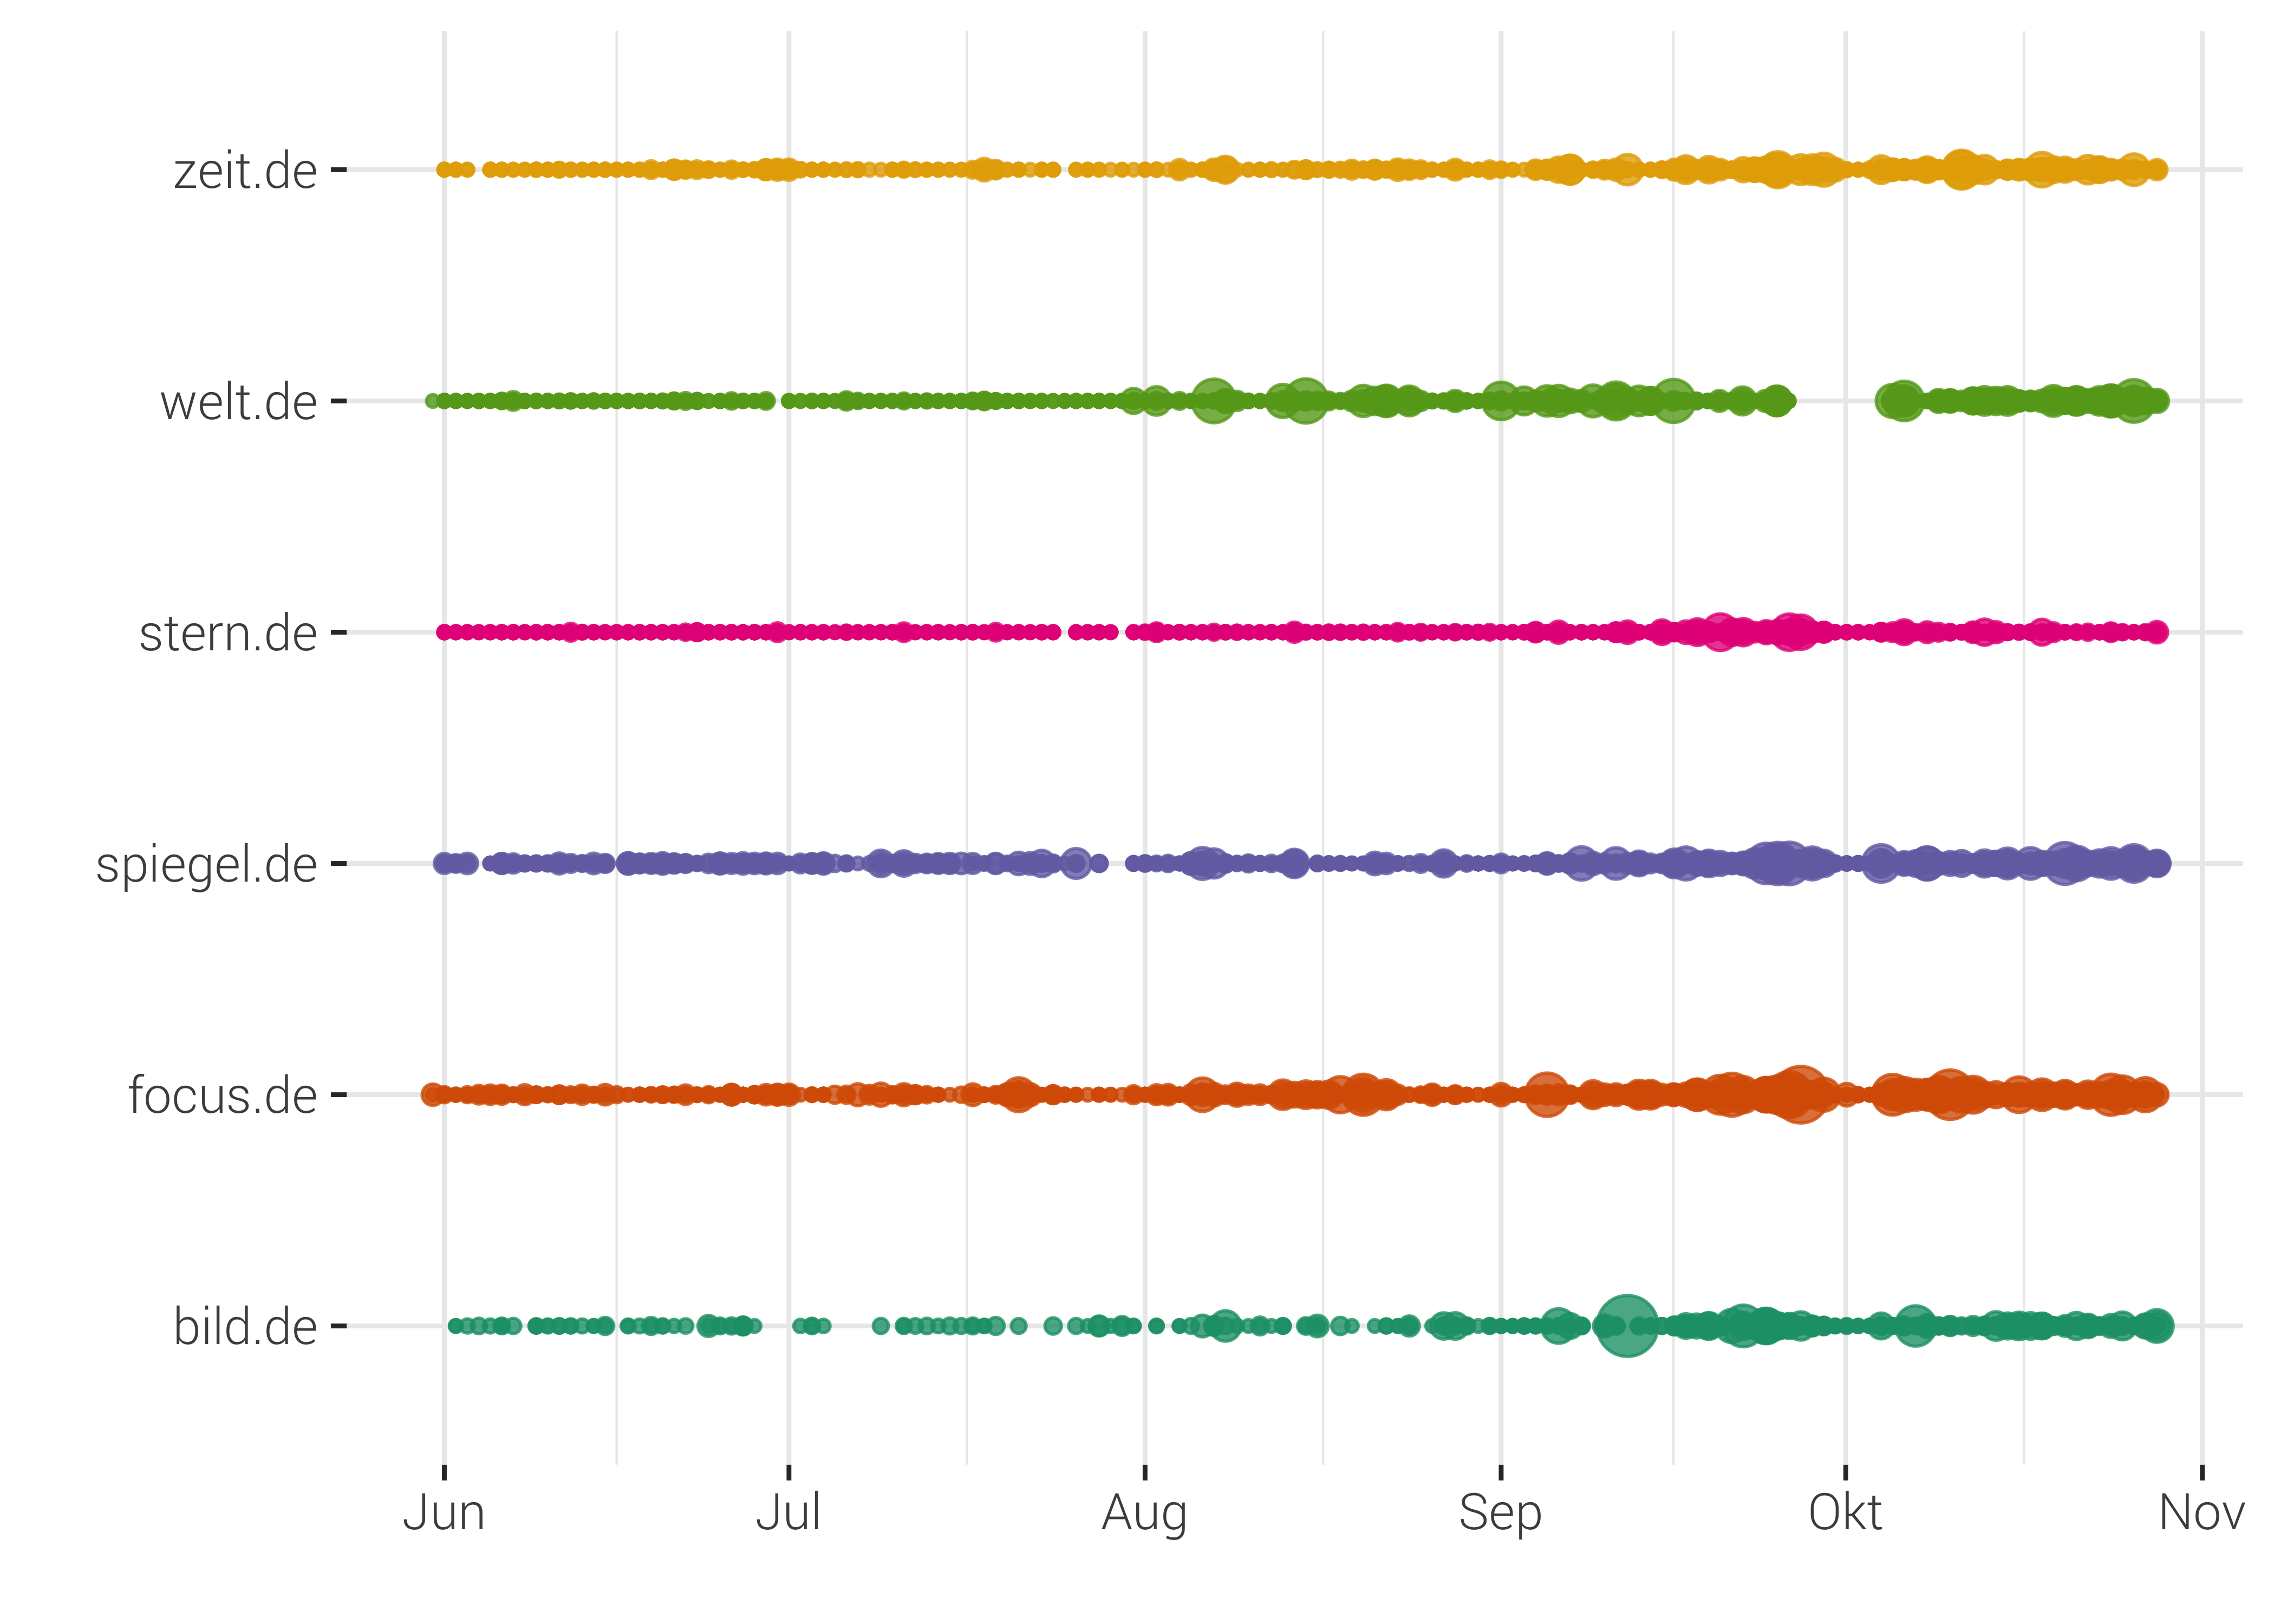
\includegraphics[width=\textwidth]{../figs/fb_shares.png}
			\caption{...by date \& news source}
		\end{subfigure}
		\begin{subfigure}[normla]{0.49\textwidth}
			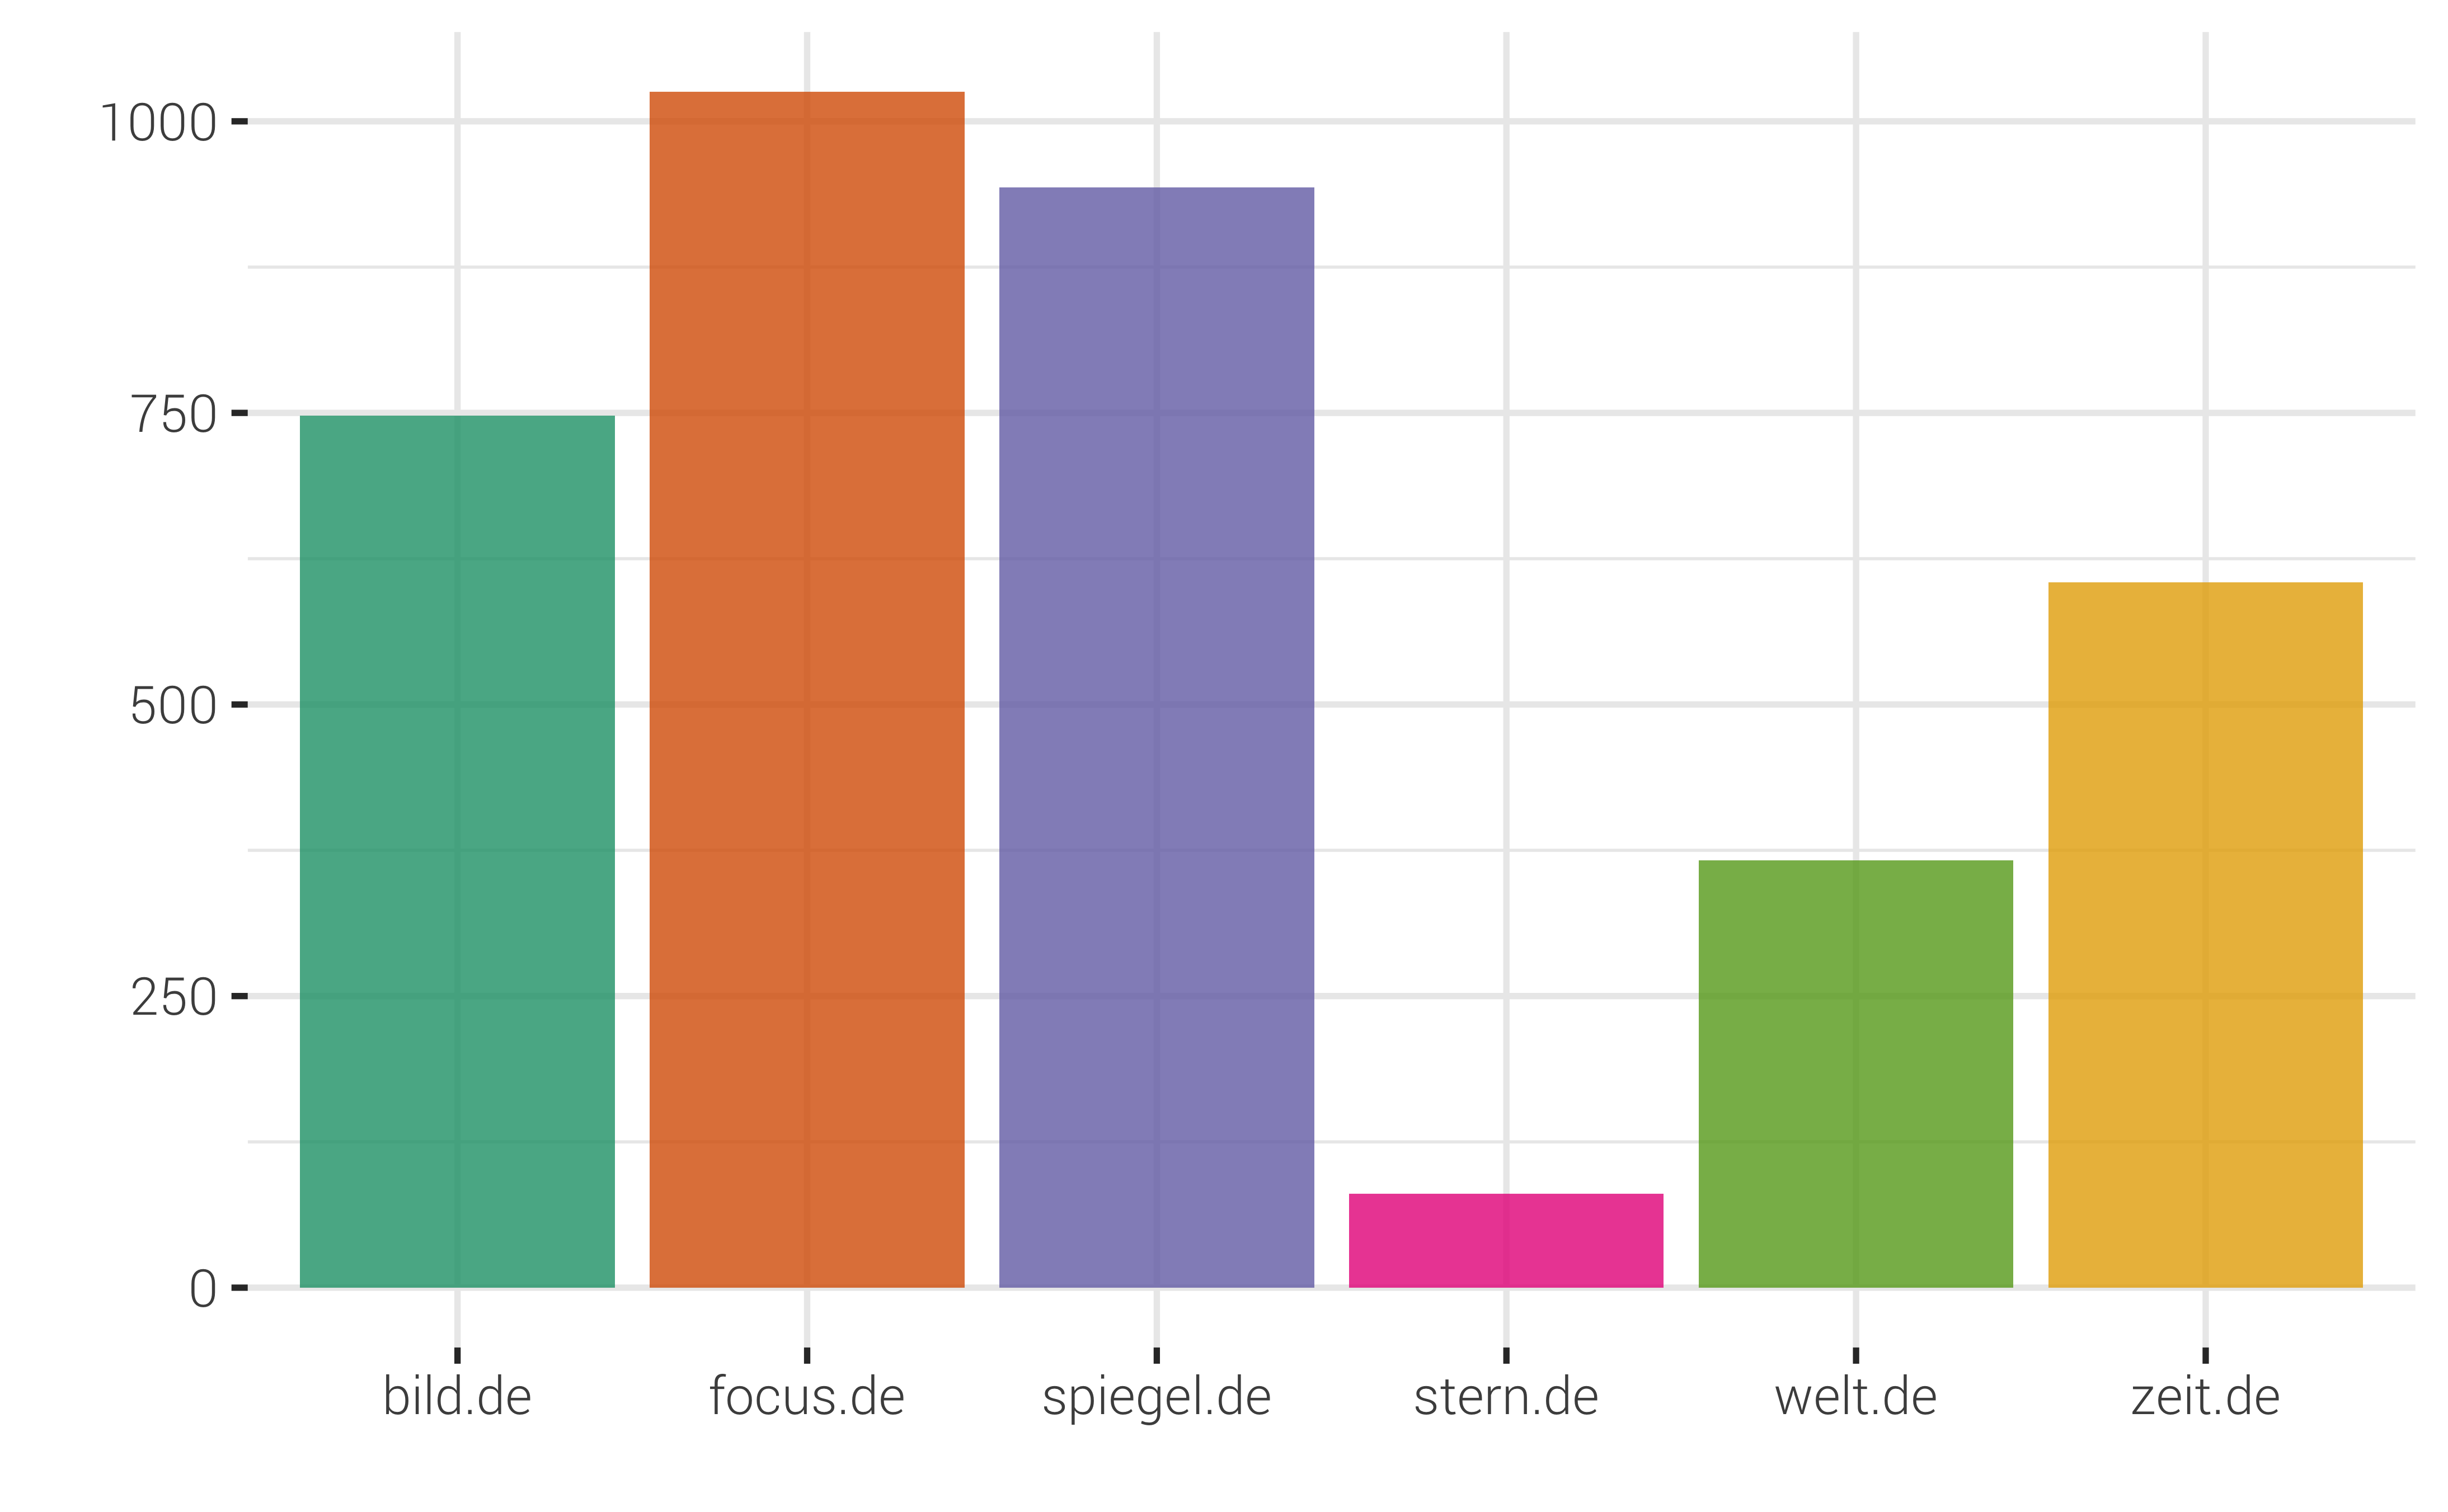
\includegraphics[width=\textwidth]{../figs/fb_shares_mean.png}
			\caption{... by news source (mean)}
		\end{subfigure}
	\end{center}
	\label{fig_fb_shares}
\end{figure}

To use text as data and reduce the dimensionality, a common strategy is to pre-process the text by imposing some preliminary restrictions (stop-word removal, tokenization) based on the nature of the data (twitter text, newspaper articles, speeches, etc.) to reduce the number of language elements to consider \citep{gentzkow_text_2017}. An overview of how these steps were applied to our data set can be found in the next section. 

After pre-processing, each document $d$ is a finite list of terms. Each unique term in the corpus is indexed by some $v \in \lbrace 1,...,V \rbrace$ where $V$ is the number of unique terms. For each document $d \in \lbrace 1,...,D \rbrace$ we compute the number of occurrences of term $v$ in document $d$ to obtain the count $x_{d,v}$. The $D$ x $V$ matrix $\boldsymbol{X}$ of all such counts is called the document-term matrix. This representation is often referred to as the bag of words model, since the order in which words are used within a document is completely disregarded. 


% ------------------
% Text Pre-Procesing
% ------------------
\subsection{Text pre-procesing and feature selection}

A central task in text mining is to extract low-dimensional information from documents that are high-dimensional by nature \citep{bholat_text_2015}. This is related to the task of reducing the number of unique language elements in order to reduce the dimensionality of data (to avoid unnecessary computational complexity and overfitting) while at the same time keeping those words that reflect the content of a document. Any useful representation of text will throw away some information, the trick is to include the relevant information for our needs, and exclude the extraneous information. 

Intuitively the term frequency (tf) of a word is a measure of how important that word may be. There are words in a document, however, that occur many times but may not be important like articles, conjunctions, and so on. These terms, often called "stop words", are important to the grammatical structure of a text, but typically don't add any additional meaning and can therefore be neglected. We use a pre-defined stop word list from the Snowball stemmer project\footnote{http://svn.tartarus.org/snowball/trunk/website/algorithms/*/stop.txt} together with a customized list of stop-words that are redundant superfluous or distorting. We also remove punctuation character (e.g. ., ,, !, ?, etc.) and all numbers from our corpus.  

We use source of each article (the news-platform) as a covariate in the topic prevalence portion of the model. Thus, we assume that the process differs with regard to the platform. In other words, the probability distribution of topics depends on the editorial strategy of a media house. We set the number of topics to be 40 after evaluating and maximizing topics' coherence using a cross-validation scheme while changing the number of topics (\citet{airoldi_reconceptualizing_2010}; \citet{roberts_model_2016}).

% ----------------------
% Structural topic Model
% ----------------------

\section{Topic detection}\label{ch_model}

As we cannot directly observe the latent topic of an article, we use an unsupervised machine learning algorithm, that takes unclassified observations of words and uncovers hidden patterns (topics) that structure them in some meaningful way. We can than use the output of this process as inputs into an econometric model, that predicts the number of Facebook shares conditional on the topic of an article \citep{gentzkow_text_2017}.  

We use the structural topic model (STM) developed by \citet{roberts_model_2016} that allows us to incorporate document specific covariates (e.g. the author or date of a document). STM is a recent extension of the standard topic modeling technique, the latent Dirichlet allocation (LDA). Topic models formalize the idea that documents are formed by hidden variables (topics) that generate correlations among observed terms. LDA is a particularly popular method for fitting a topic model \citep{blei_latent_2003}, also known as the generative aspect model \citep{minka_expectation-propagation_2002}. Each document $d$ is generated from the following process \citep{blei_latent_2003}: The number of words $N$ is a random  , containing $N_d$ words from a vocabulary of interest of $V$ unique terms, is a mixture of $k$ topics. Thus, each document has its own probability distribution over topics. Simultaneously, each topic has a probability distribution over terms, associated with a $V$-dimensional probability mass function $\boldsymbol{\beta}_k$, that controls the frequency according to which terms are generated from that topic. 

This standard topic modeling technique makes the assumption that all texts in the modeled corpus are generated by the same underlying process \citep{mishler_using_2015}. To include additional information that improve the estimation of the topics, we estimate a structural topic model, where topical prevalence (the distribution of topics among documents) is specified as a simple generalized linear model on document-level metadata. 

The following description of the generative model of the STM is based on \citet{roberts_structural_2013} ans \citept{roberts_stm:_2016}. The process of filling a word-position in a document begins with the generation of a document-specific topic-prevalence vector $d(\boldsymbol{\theta}_d)$ drawn from a logistic-normal distribution, where the parameters are a function of the covariate values:

\begin{align*}
	\boldsymbol{\theta}_d|\boldsymbol{x}_{d\gamma},\boldsymbol{\Sigma} \sim \textrm{LogisticNormal}(\mu = \boldsymbol{x}_{d\gamma}\boldsymbol{\Sigma})
\end{align*}

$\boldsymbol{x}_d\gamma$ lists the values of all metadata covariates for document $d$, where $\gamma$ relates these covariate values to the topic-prevalence. The structure of $\boldsymbol{\Sigma}$ implies the possibility of correlations across documents in the topic-prevalence vector which help enhance interpretation and prevent overfitting. 

Given the document-specific distribution over topics, for each word in the document ($n \in \lbrace 1,...,N_d\rbrace$) is assigned to a specific topic $z_{dn}$ through the process

\begin{align*}
	z_{dn}|\boldsymbol{\theta}_d \sim \textrm{Multinomial}(\boldsymbol{\theta}_d)
\end{align*}

where the $k^{th}$ element if $z_{dn}$ is unity and all other elements are zero when topic $k$ is chosen. 

Conditional in the topic chosen, a specific word, $w_{dn}$, is chosen from the overall corpus vocabulary $V$ to fill position $n$ in document $d$, using the following process:

\begin{align*}
	w_{dn}|z_{dn},\beta_{dkv} \sim \textrm{Multinomial}(\beta_{dk1},...,\beta_{dkV}).
\end{align*}

where the word probability $\beta_{dkv}$ is modeled as a function of the two parameters $m_v$ (indicating the importance of that word across all documents) and $\kappa_{kv}$ (indicating the importance of the word given the topic $k$). Transforming the sum of these coefficients into probabilities for use in a multinomial distribution via logistic transformation, one obtains:

\begin{align*}
	\beta_{dkv}|z_{dn}\propto\textrm{exp}(\boldsymbol{m}_v+\kappa_{kv})
\end{align*}


The STM maximizes the posterior likelihood that the observed data were generated by the above data-generating process using an iterative approximation-based variational expectation-maximization algorithm available in R's stm package \citep{roberts_stm:_2016}. Regularizing prior distributions are used for $\gamma$, $\kappa$ and (optionally) $\Sigma$. To address problems due to non-convexity, we rely on the spectral initialization approach advocated by \citet{roberts_navigating_2016}.

\section{Probabilities and Classification}\label{ch_results}

After performing the topic modeling, we can generate an overview of the news landscape about the german elections. Each group is composed of the most relevant words for that topic, and a manually-determined label. The distances that the topics have from each other reflect their semantic distance, or basically how different the words are for that topic. It is computed as the Jensen-Shannon divergence between each of the topics according to the differences in their word-topic probabilities. We then apply principal coordinates analysis in order to project the distance matrix down to two dimensions.

%\begin{figure}[H]
%\centering
%	\caption{News Landscape}
%	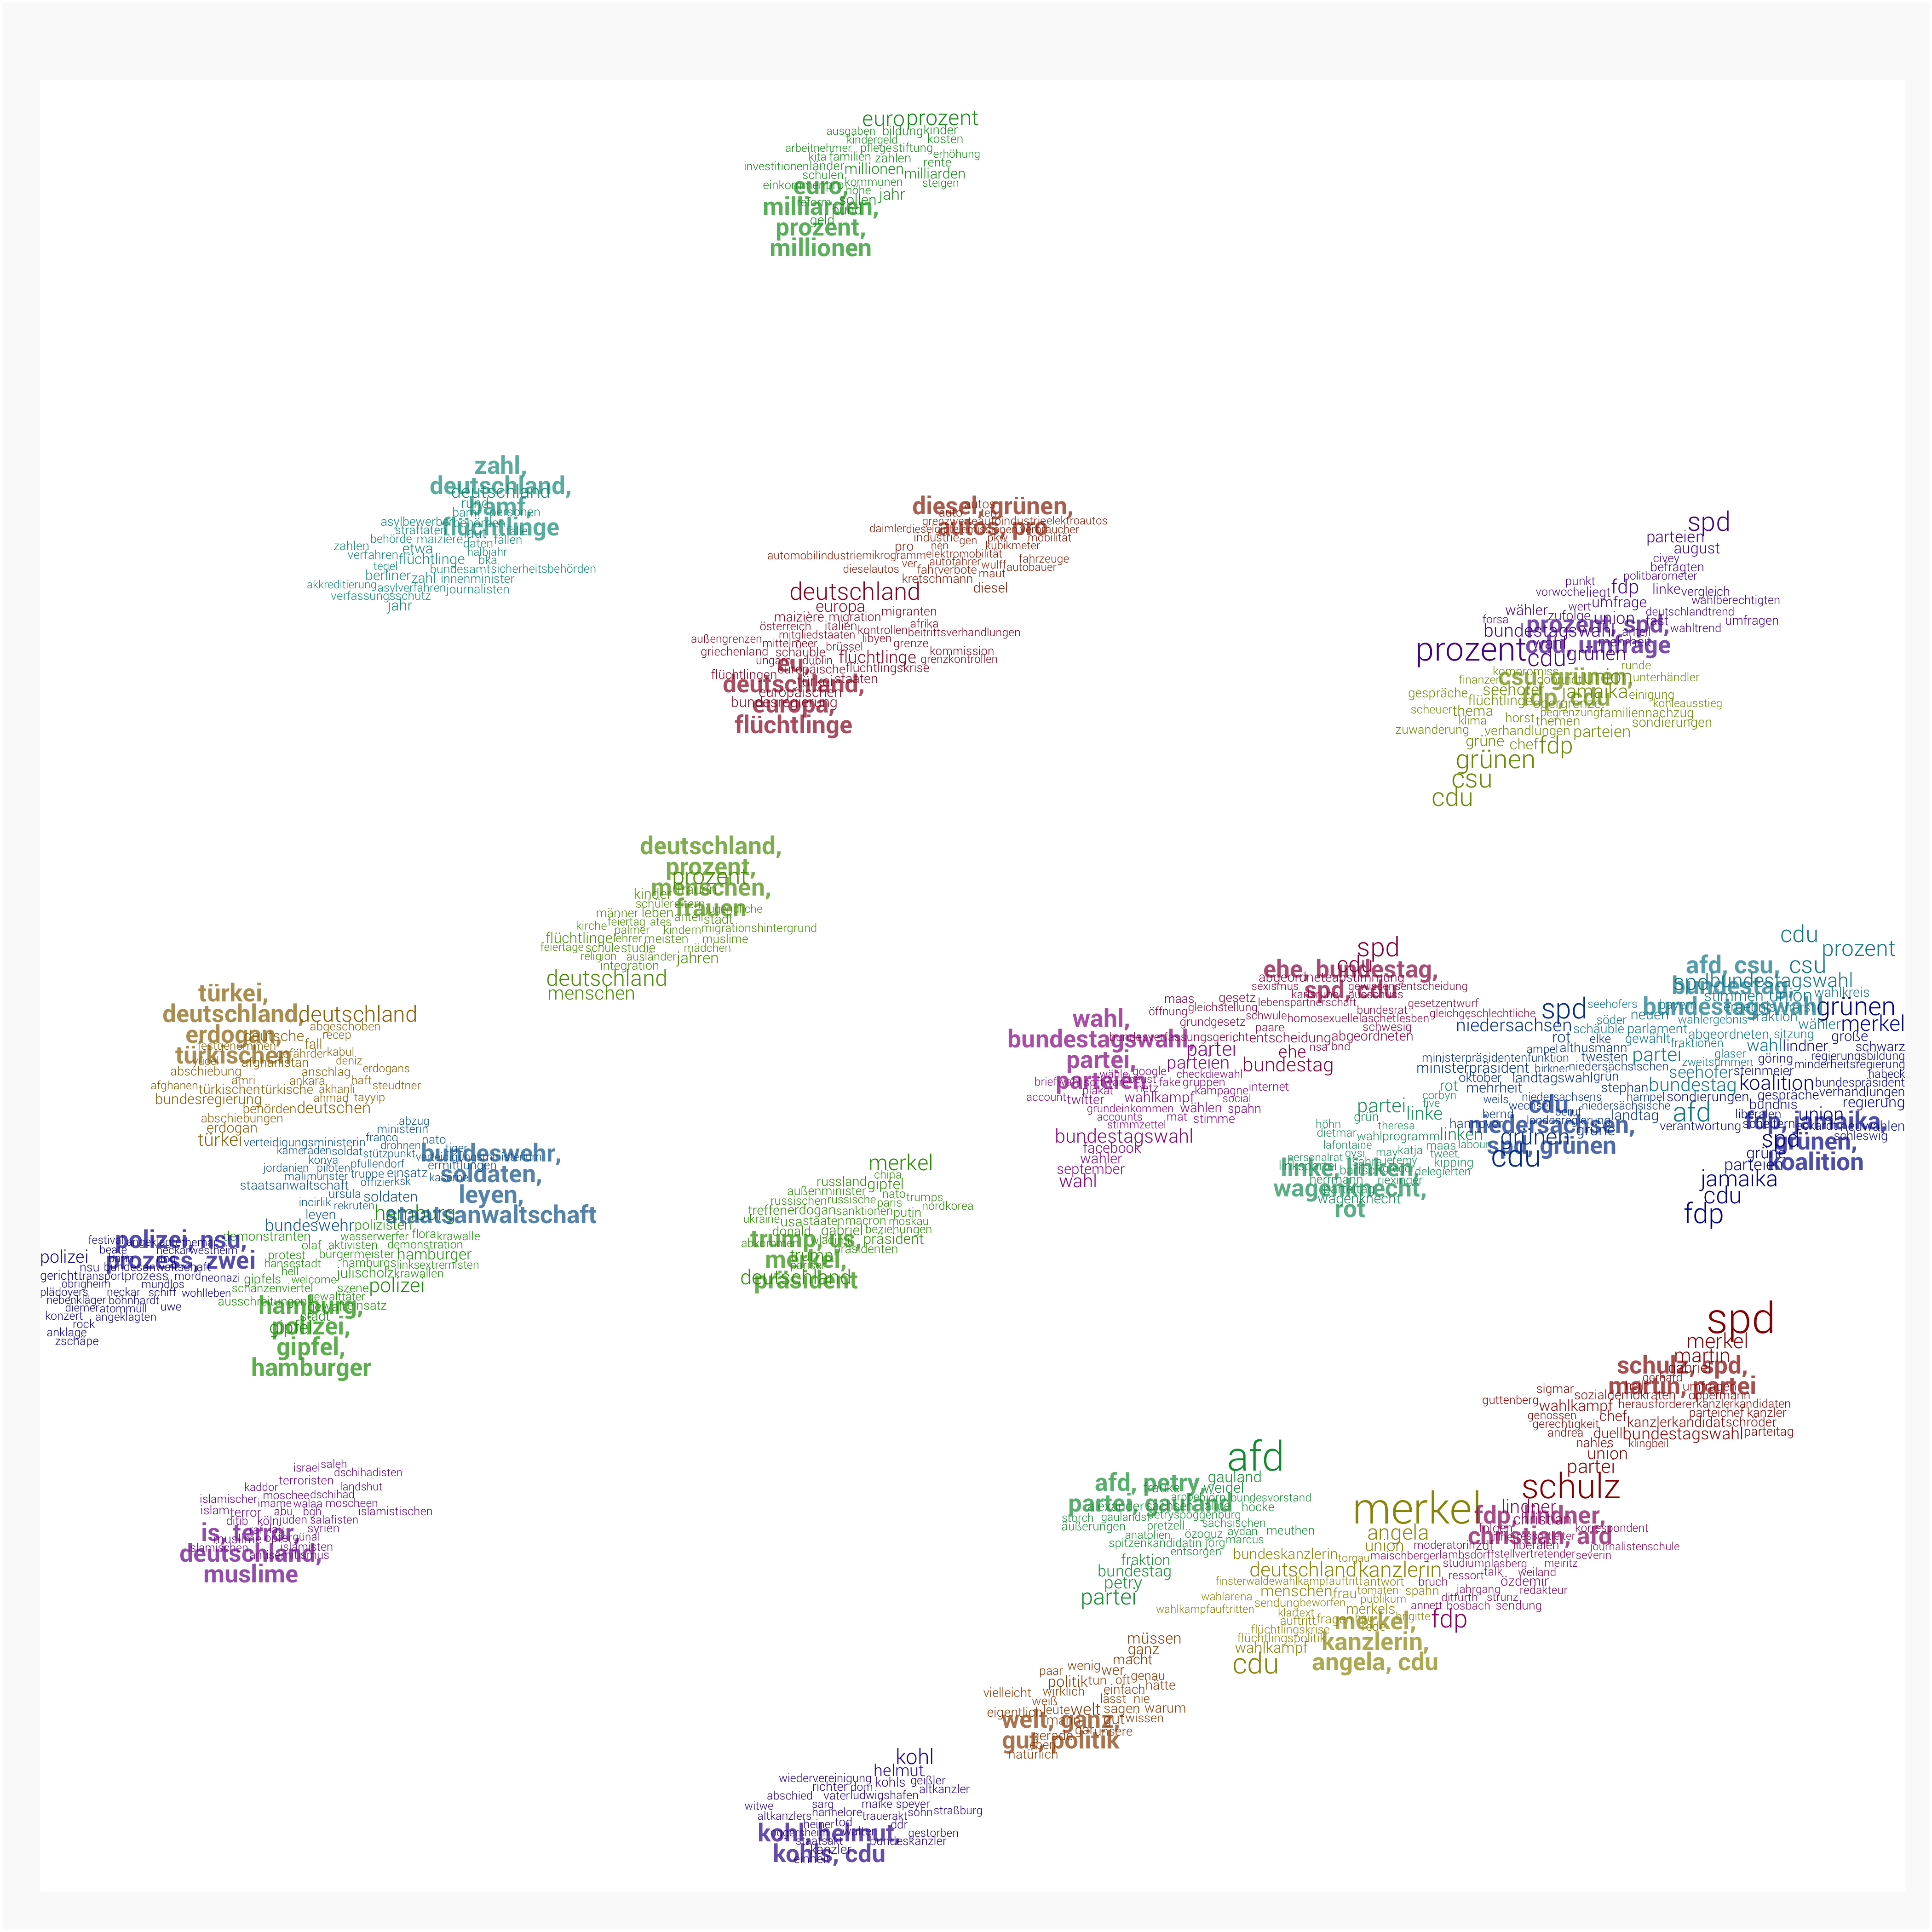
\includegraphics[width=\textwidth]{../figs/news-landscape-map.png}	
%	\label{fig_landscape}
%\end{figure}

To check weather the estimated topic classifications make sense, we first produce sample documents classified to that topic for reference. We produce a random sample of 10 posts from the 300 highest probability fits per topic.

%\begin{figure}[H]
%\centering
%	\caption{Sample articles}
%	\includegraphics[width=\textwidth]{../figs/topic-classification-sample.png}	
%	\label{fig_classification}
%\end{figure}
%
%\begin{figure}[H]
%\centering
%	\caption{Sum of Facebook shares by topic}
%	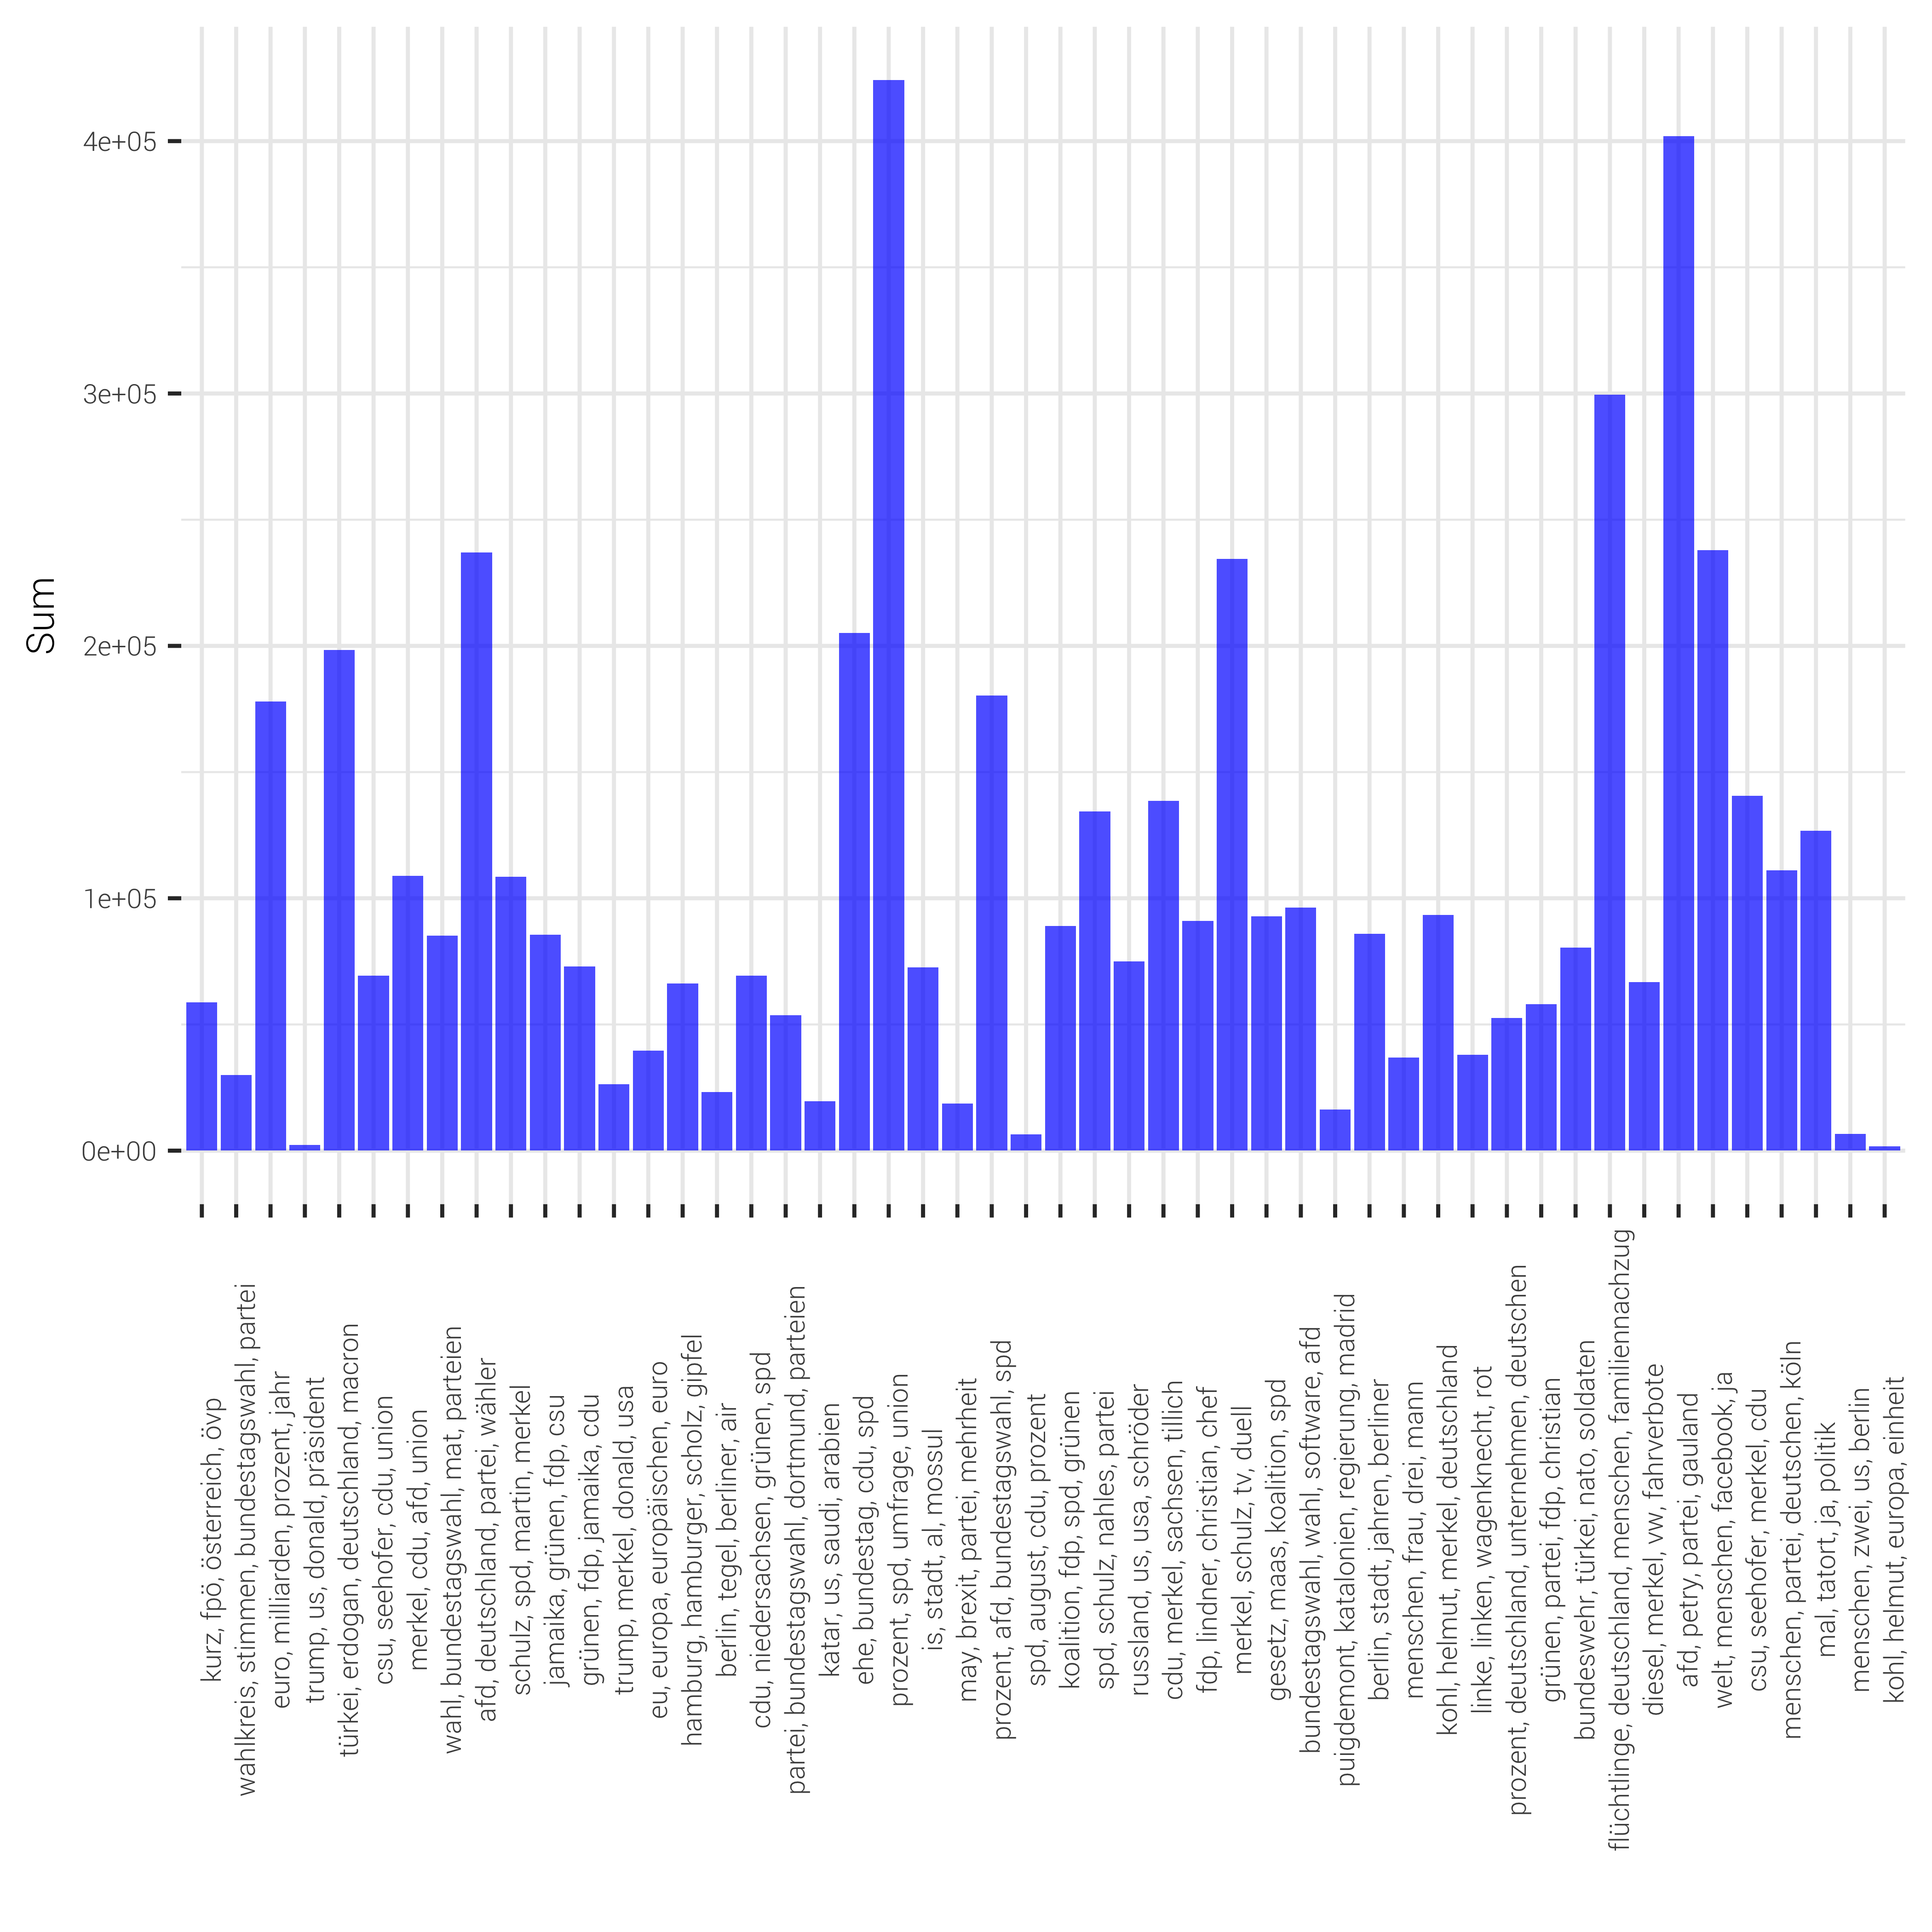
\includegraphics[width=\textwidth]{../figs/fb_shares_topics.png}	
%	\label{fig_fb_shares_topic}
%\end{figure}

\section{Regression}\label{ch_regression}

The examination of the topic probability distribution revealed that most documents are assigned a unique topic with high probability (65\% and higher), so that we can classify each document based on which topic has the highest probability. We keep only those documents, where the posterior probability of this topic is greater than 0.6 which left us with 6240 documents. 

The proportion of zeros in the independent variable (number of Facebook shares) is about 66\%. One way to model this type of situation is to assume that the data come from a mixture of two populations, one where the counts is always zero, and another where the count has a Poisson distribution with mean $\mu$. In this model zero counts can come from either population, while positive counts come only from the second one. 

The distribution of the outcome can then be modeled in terms of two parameters, $\pi$ the probability of 'always zero', and $\mu$, the mean number of publications for those not in the 'always zero' group. A natural way to introduce covariates is to model the logit of the probability $\pi$ of always zero and the log of the mean $\mu$ for those not in the always zero class.

The two-part model relaxes the assumption that the zeros (whether or not the article is shared) and positives (how often it is shared) come from the same data generating process. The zero-inflated model lets the zeros occur in two different ways: as a realization of the binary process (z=0) and as a realization of the count process when the binary variable z=1. 

If the process generating the zeros is $f_1(.)$ and the process generating the positive responses is $f_2(.)$ then the two-part hurdle model is defined by the following probabilities. 

\begin{align*}
	g(y)=\begin{cases}
		f_1(0) + 1(f_i(0))f_2(0) if y=0 \\
		(1-f_1(0))f_2(y) if y\geq 1
	\end{cases}
\end{align*}

The model for the zero versus positive responses is a binary model with the specified distribution, but we usually estimate it with the probit/logit model.

\end{document}
